\documentclass[12pt, onside]{article}
\usepackage[utf8]{inputenc}             % UTF8 encoding
\usepackage{parskip}% Extra interlining
\usepackage[margin=0.8in]{geometry}    % Margins
\usepackage[spanish]{babel}


% Header and Footer
\usepackage{fancyhdr}
\setlength\headheight{30pt}
\pagestyle{fancy}
\renewcommand{\headrulewidth}{0.4pt}
\fancyhead{}
\fancyhead[L]{
    \textbf{Prácticas Servicios Telemáticos}
}
\fancyhead[R]{
    Emilio Domínguez Sánchez
}
\fancyfoot{}
\fancyfoot[C]{\thepage}


\usepackage{hyperref}
\usepackage{cleveref}
\usepackage{xcolor}
\usepackage{graphicx}
% Code Listings Configuration File

\usepackage{listings}
\renewcommand{\lstlistingname}{Código}
\crefname{lstlisting}{código}{códigos}
\Crefname{lstlisting}{Código}{Códigos}


\definecolor{background}{rgb}{0.99,0.99,0.99}
\definecolor{mygreen}{rgb}{0.1,0.6,0.1}
\definecolor{mygray}{rgb}{0.5,0.5,0.5}
\definecolor{mymauve}{rgb}{0.58,0,0.82}

\definecolor{codeback}{rgb}{0.85,0,0.85}
\newcommand{\code}{\lstinline[basicstyle=\selectfont, language=C]}

\renewcommand{\lstlistlistingname}{Índice de códigos}
\lstset{ 
  title=Fichero \lstname,          % show the filename of files included with \lstinputlisting; also try caption instead of title
  caption=Fichero \texttt{\lstname},
  captionpos=t,                    % sets the caption-position (b/t)
  frame=TBLR,      	               % adds a frame around the code
  rulecolor=\color{black},         % if not set, the frame-color may be changed on line-breaks within not-black text (e.g. comments (green here))
  numbers=left,                    % where to put the line-numbers; possible values are (none, left, right)
  numbersep=10pt,                  % how far the line-numbers are from the code
  % stepnumber=1,                    % the step between two line-numbers. If it's 1, each line will be numbered
  backgroundcolor=\color{background},
  numberstyle=\small\color{mygray},% the style that is used for the line-numbers
  basicstyle=\scriptsize\selectfont, % the size/type of the fonts that are used for the code
  keywordstyle=\color{blue},       % keyword style
  commentstyle=\color{mygreen},    % comment style
  stringstyle=\color{mymauve},     % string literal style
  breakatwhitespace=false,         % sets if automatic breaks should only happen at whitespace
  breaklines=true,                 % sets automatic line breaking
  keepspaces=true,                 % keeps spaces in text, useful for keeping indentation of code (possibly needs columns=flexible)
  showstringspaces=false,          % underline spaces within strings only
  showspaces=false,                % show spaces everywhere adding particular underscores; it overrides 'showstringspaces'
  showtabs=false,                  % show tabs within strings adding particular underscores
  tabsize=2,	                   % sets default tabsize to 2 spaces
  language=C++,                    % the language of the code
  morekeywords={},            % if you want to add more keywords to the set
  deletekeywords={},            % if you want to delete keywords from the given language
  % escapeinside={----}{----},          % if you want to add LaTeX within your code
  extendedchars=true,              % lets you use non-ASCII characters; for 8-bits encodings only, does not work with UTF-8
  literate=
  {á}{{\'a}}1 {é}{{\'e}}1 {í}{{\'i}}1 {ó}{{\'o}}1 {ú}{{\'u}}1
  {Á}{{\'A}}1 {É}{{\'E}}1 {Í}{{\'I}}1 {Ó}{{\'O}}1 {Ú}{{\'U}}1
  {à}{{\`a}}1 {è}{{\`e}}1 {ì}{{\`i}}1 {ò}{{\`o}}1 {ù}{{\`u}}1
  {À}{{\`A}}1 {È}{{\'E}}1 {Ì}{{\`I}}1 {Ò}{{\`O}}1 {Ù}{{\`U}}1
  {ä}{{\"a}}1 {ë}{{\"e}}1 {ï}{{\"i}}1 {ö}{{\"o}}1 {ü}{{\"u}}1
  {Ä}{{\"A}}1 {Ë}{{\"E}}1 {Ï}{{\"I}}1 {Ö}{{\"O}}1 {Ü}{{\"U}}1
  {â}{{\^a}}1 {ê}{{\^e}}1 {î}{{\^i}}1 {ô}{{\^o}}1 {û}{{\^u}}1
  {Â}{{\^A}}1 {Ê}{{\^E}}1 {Î}{{\^I}}1 {Ô}{{\^O}}1 {Û}{{\^U}}1
  {œ}{{\oe}}1 {Œ}{{\OE}}1 {æ}{{\ae}}1 {Æ}{{\AE}}1 {ß}{{\ss}}1
  {ű}{{\H{u}}}1 {Ű}{{\H{U}}}1 {ő}{{\H{o}}}1 {Ő}{{\H{O}}}1
  {ç}{{\c c}}1 {Ç}{{\c C}}1 {ø}{{\o}}1 {å}{{\r a}}1 {Å}{{\r A}}1
  {€}{{\euro}}1 {£}{{\pounds}}1 {«}{{\guillemotleft}}1
  {»}{{\guillemotright}}1 {ñ}{{\~n}}1 {Ñ}{{\~N}}1 {¿}{{?`}}1
}

\usepackage[binary-units=true]{siunitx}
\usepackage{multirow}



\newcommand{\key}{\texttt}
\newcommand{\file}{}
\newcommand{\HTTP}{HTTP}
\newcommand{\GET}{GET}
\newcommand{\POST}{POST}
\newcommand{\HTML}{HTML}
\newcommand{\TCP}[0]{TCP}
\newcommand{\Clang}{C}
\newcommand{\Cplusplus}{C++}



\begin{document}
\begin{titlepage}
    \begin{center}
        \vspace*{1cm}
        
        \Huge \textbf{Servicios Telemáticos}
        
        \vspace{0.5cm}
        \LARGE Práctica Final
        
        \vspace{0.5cm}
        
        \Large Entrega Anticipada
        
        \vspace{0.5cm}
   		
        \vfill
        
        %Obor XY
        \vspace{0.8cm}
        \Large
            \begin{flushright}
              	\begin{tabular}{lr}
                  Autor:        & Emilio Domínguez Sánchez\\
                  Convocatoria: & Junio 2020\\
                  Grupo:        & 1.4 \\
                \end{tabular}
            \end{flushright}
        \vspace{0.5cm}
        
    \end{center}
\end{titlepage}

\newpage
\tableofcontents
\newpage

\section{Introducción}
La asignatura de Servicios Telemáticos del grado en Ingeniería Informática consta de una parte práctica que consiste en configurar y poner en marcha un conjunto de servicios telemáticos. El enunciado de la práctica %TODO referencia
describe los objetivos. En esta memoria se recoge la implementación del enunciado así como el proceso de toma de decisiones.


%\section{Escenario Desarrollado y Versiones del Software}
%\section{Configuraciones}

\section{Servidor Web \HTTP}
\subsection{Introducción}
Implementar y desplegar un servidor {\HTTP} es la tarea principal de estas prácticas. De aquí en adelante, cuando hablemos del servidor nos referiremos a la implementación en lenguaje {\Clang} que hemos llevado a cabo.


\subsection{Usos de \Cplusplus}
Como comentaba, este apartado de prácticas debía realizarse en \Clang. Sin embargo, comenté con mi profesor de prácticas la posibilidad de utilizar \Cplusplus utilizando las mismas llamadas al sistema. Sin embargo, para cumplir con los requisitos de la entrega he mantenido el código como si fuese \Clang. En ese sentido, el grueso del programa es código \Clang. En concreto, he utilizado \Cplusplus para

\begin{itemize}
\item Una clase para imprimir los registros. Permite escribir al registro utilizando la sintaxis que muestro en el \cref{lst-log}.

\item Y en algunas funciones para pasar algunos valores por referencia. Cuando se quiere pasar por referencia un puntero en \Clang, la sintaxis no es cómoda.
\end{itemize}

\begin{lstlisting}[caption=Uso de las clases \code{log} y \code{logerr}, label=lst-log]
Code:   log << "alberto, tenemos un problema de tipo " << type << endl;
Output: INFO(socket ---): alberto, tenemos un problema de tipo ---
Code:   log << endl;
Output:
Code:   log << "mensaje de log 1" << endl;
        log << "mensaje de log 2\n";
Output: INFO(socket ---): mensaje de log 1
        INFO(socket ---): mensaje de log 2
Code:   logerr << "falló una llamada al sistema" << endl;
Output: ERROR: errno=--- exiting pid=---: falló una llamada al sistema
Code:   logerr << "problemas Mike!" << endl << panic();
Output: ERROR: errno=--- exiting pid=---: problemas Mike!
-> Program finishes execution with code -1
\end{lstlisting}


\subsection{Inicio del servidor}
El objetivo básico de un servidor web http es recibir peticiones, que vendrán en forma de un mensaje \key{HTTP request}, y tratarlas. Normalmente, tratarlas significa devolver un recurso al que se intenta acceder.

La función \code{main} del servidor se encuentra dentro del fichero \file{main.cpp}. Al inicio del programa (\cref{lst-daemon}), el objetivo es que el servidor sea ejecutado desde la terminal y funcione como un demonio (es decir, en segundo plano). Para ello, creamos un hijo e ignoramos la señal \key{SIGHUP}% a footnote follows
\footnote{La señal \key{SIGHUP} es una señal que se envía a un proceso cuando la terminal que lo controla finaliza.}.
El proceso padre finaliza automáticamente para devolver el control a la terminal.

\lstinputlisting[linerange={48-59}, label=lst-daemon]{src/main.cpp}

Cuando el servidor recibe una nueva conexión {\TCP} de un cliente, crea un proceso hijo que se encarga de atenderlo y espera hasta recibir otra conexión (\cref{lst-parent-behaviour}).

\lstinputlisting[linerange={61-91}, label=lst-parent-behaviour]{src/main.cpp}

\subsection{Intercambio de mensajes}
La complejidad del servidor está en el trabajo que realiza el proceso para atender al cliente. La función {\Clang} que maneja la conversación es \code{deal_with_client}.

% Apreciaciones Técnicas:
\begin{itemize}
\item Para la lectura se utiliza un buffer de \SI{8}{\kibi\byte}. El servidor lee (\cref{lst-header-reading}) datos de la conexión {\TCP} hasta completar la cabecera de un mensaje {\HTTP} (indicada por la secuencia \code{"\r\n\r\n"}).

\item Tras completar la cabecera de un mensaje, se interpreta la primera línea, llamada \key{status-line} en el protocolo {\HTTP}, para determinar el tipo de mensaje y llamar a una función que lo procese (\cref{lst-request-line}). Esto implica que la cabecera ha de caber en el buffer. Es decir, hay un límite de \SI{8}{\kibi\byte} para el tamaño de la cabecera; y el servidor enviará un mensaje de error en caso de que se supere este tamaño. En la práctica es más que suficiente. Ningún mensaje, aún usando todos los campos disponibles en el protocolo {\HTTP}, utilizaría tanto espacio.

\item El servidor acepta mensajes de tipo {\GET} y {\POST}. Del campo de cabecera \key{content-length} obtiene el tamaño del cuerpo del mensaje, que incorpora al buffer.

\item El servidor no conoce el tamaño de la cabecera de antemano, lo que significa que es posible leer más bytes que los que ocupa un mensaje% a footnote follows
\footnote{Enviar dos mensajes antes de recibir la respuesta del primero se llama \key{pipelining}. Según nuestras pruebas, la versión de \code{firefox} que utilizamos en la máquina virtual no implementa \key{pipelining}.}.
Las funciones \code{process_get} y \code{process_post} devuelven un referencia al primer byte que no formaba parte de su mensaje. La función \code{deal_with_client} lo utiliza para completar la cabecera del siguiente mensaje. De esta manera, la función \code{deal_with_client} no necesita inspeccionar la cabecera (\cref{lst-buffer-adaptation}).
\end{itemize}

\lstinputlisting[linerange={368-408}, label=lst-header-reading]{src/message_processing.cpp}
\lstinputlisting[linerange={418-431}, label=lst-request-line]{src/message_processing.cpp}
\lstinputlisting[linerange={433-450}, label=lst-buffer-adaptation]{src/message_processing.cpp}


\subsection{Persistencia}
Como comentábamos en la sección anterior, el servidor está preparado para aceptar más de un mensaje en la misma conexión. Es lo que se conoce como persistencia en el protocolo {\HTTP}. Las funciones que inspeccionan la cabecera comprueban si el cliente busca mantener la conexión según el valor de la línea de cabecera \key{Connection} y la versión {\HTTP} (el protocolo \key{{\HTTP}/1.0} no se diseñó enfocado a persistencia).

El servidor se ha configurado con un timeout de \SI{5}{\second} que anuncia en la cabecera \key{Keep-Alive}. Se trata del máximo tiempo que el servidor mantendrá la conexión abierta antes de recibir el primer byte del siguiente mensaje (como especifica el protocolo). No obstante, incurrimos en un riesgo de bloqueo si no incluimos otro timeout cuando se espera para completar un mensaje. Un cliente malintencionado podría dejar una conexión abierta indefinidamente, lo que se traduce en un riesgo de negación de servicio (\key{DoS}). Por tanto, hemos incluido un timeout de \SI{1}{\second}.

\subsubsection{Tiempos de timeout en la lectura de cabecera}
Para el control de los tiempos de timeout hemos utilizado la llamada al sistema \code{select} de linux. Es una directiva de sincronización que permite bloquearse a la espera de datos de un \key{socket} durante un tiempo determinado.

La implementación del timeout entre mensajes se puede ver en el \cref{pre-header-timeout}. Es importante ver que hay una comprobación antes sobre el tamaño del buffer de lectura. El motivo es el que ya hemos comentado. Puede ser que hayamos leído parte del mensaje siguiente (incluso entero), en cuyo caso no tenemos por qué esperar.

La implementación del timeout para completar la cabecera se puede ver el \cref{header-timeout}. En ambos casos, si el cliente no envía datos en el tiempo establecido se aborta la conexión. En el caso de que no haya comenzado un mensaje, se trata de un corte normal. En cambio, si ya había comenzado el mensaje y no nos ha llegado el resto del mensaje puede ser que la conexión funcione mal o que sea el cliente el que funcione incorrectamente. En cualquier caso, cortamos la conexión y terminamos con un código de error.

\lstinputlisting[linerange={356-367}, label=pre-header-timeout]{src/message_processing.cpp}
\lstinputlisting[linerange={382-382, 399-407}, label=header-timeout]{src/message_processing.cpp}

\subsubsection{Tiempos de timeout en la lectura del cuerpo del mensaje}
Para aquellos mensajes que contienen un cuerpo (mensajes {\POST} principalmente) también tenemos que controlar el timeout si intentamos leer más datos. Si no, corremos el riesgo de mantener un hilo infinitamente abierto ante un error o un cliente malintencionado. Se hace de forma similar al \cref{header-timeout} pero dentro de las funciones \code{process_get} y \code{process_post}.

\subsubsection{Manejo de las cabeceras \key{Connection} y \key{Keep-Alive}}
El protocolo {\HTTP} exige al servidor que informe al cliente si va a mantener la conexión abierta y cuánto tiempo asegura que lo hará% a footnote
\footnote{Aunque el servidor intente mantener siempre la conexión abierta, puede no poder hacerlo por dos motivos. Porque el cliente pida mantenerla cerrada o porque haya que abortar la conexión, por ejemplo tras un error de formato.}
. Lo primero se hace a través de la cabecera \key{Connection}, que puede tomar los valores \key{close} o \key{keep-alive}. El tiempo se especifica en la cabecera \key{keep-alive}. En nuestra implementación, las funciones que envían ficheros reciben un parámetro que indica si la conexión se mantendrá abierta.

\subsection{Métodos {\GET} y {\POST}}
La funciones \code{process_get} y \code{process_post} inspeccionan del buffer de lectura un mensaje (tipo {\GET} o {\POST}), leen datos del socket hasta completar el cuerpo del mensaje y devuelven el recurso que pide el cliente en forma de un mensaje \key{{\HTTP} response}. En caso de que el mensaje no cumpla el formato o se produzca un error, se devuelve el mensaje de error que indique el protocolo y dependiendo del caso se aborta la ejecución.

Hemos aplicado el siguiente criterio para el corte de la conexión. Si el error es de formato, se considera que no se puede determinar dónde acabaría el mensaje y empezaría el siguiente, y por tanto se aborta la conexión. Lo mismo sucede si se produce un error interno; por ejemplo, por un fallo de una llamada al sistema. En cambio, un error como intentar acceder a un recurso que no existe se considera un error leve. Se devolvería un mensaje con el famoso código {\HTTP}, \key{404 Not Found}, y se procesaría el siguiente mensaje. Se puede ver la implementación de la función \code{process_get} en el \cref{lst-process-get}.

\lstinputlisting[linerange={183-253}, label=lst-process-get]{src/message_processing.cpp}

La función \code{process_post} se comporta de manera similar a la hora de inspeccionar la cabecera, pero la funcionalidad es limitada. Al tratarse de un proyecto de prácticas, el contenido de prueba del servidor solo contiene un formulario {\HTML}. Si se recibe la cadena \code{"email=emilio.dominguezs%40um.es"} devuelve una página de felicitación (\cref{lst-post-check}).

\lstinputlisting[linerange={331-337}, label=lst-post-check]{src/message_processing.cpp}


\subsection{Mensajes {\HTTP} Response}
La función \code{send_static_file} envía un fichero del sistema a través de un mensaje {\HTTP}. Es una función genérica a la que llaman \code{process_get}, \code{process_post} y otras funciones que envían mensajes de error (como \code{send_bad_request}).

La función utiliza un buffer de escritura de $2\cdot \SI{8}{\kibi\byte}$ para poder hacer lecturas (de disco) y escrituras de \SI{8}{\kibi\byte} y minimizar las llamadas al sistema.

\begin{itemize}
\item Mientras el buffer no contenga más de \SI{8}{\kibi\byte} y no se haya leído el fichero al completo, se hace una operación de lectura de \SI{8}{\kibi\byte} del fichero (la operación puede leer menos datos). Como el buffer es de $2\cdot\SI{8}{\kibi\byte}$, siempre hay espcacio para los datos.

\item Mientras el buffer contenga más de \SI{8}{\kibi\byte} o el fichero se haya leído completamente y queden datos por enviar, se ejecuta una operación de escritura de \SI{8}{\kibi\byte}. A continuación se desplaza el exceso de datos al comienzo del buffer para mantener todo el espacio libre a continuación del espacio usado.
\end{itemize}

\lstinputlisting[linerange={15-30,101-181}, label=lst-send-static]{src/message_processing.cpp}

\subsection{Otras anotaciones sobre el código fuente}
Esta sección está dedicada a partes del código que no forman parte de la lógica principal del programa.

\begin{itemize}
\item El fichero \file{http\_parsing.cpp} contiene funciones que sirven para separar los campos de un mensaje {\HTTP}. El mensaje original se modifica y se insertan caracteres nulos en el lugar de algunos delimitadores y se devuelven referencias al caracter donde empezaba cada campo. Como se mantienen referencias al mensaje original, el código es muy eficiente, pero al leer información en el buffer encima de la información actual las referencias se vuelven inválidas. Las funciones también comprueban fallos en el formato de la cabecera.

\item El fichero \file{defs.hpp} contiene definiciones generales para el servidor. Por ejemplo, permite a un usuario cambiar los tiempos de timeout o las asociaciones \key{MIME} que identifican el tipo de fichero según su extensión.
\end{itemize}

\subsection{Mejoras}
Esta sección está pendiente. En la entrega de final incluirá las mejoras que se hayan implementado.
%TODO


\subsection{Ejemplos de funcionamiento y capturas del tráfico de red}
En el archivo \file{tests/capture-global.pcapng} se muestra una captura del funcionamiento del servidor tomada con Wireshark. En las fotos que presentamos hemos aplicado el filtro
\begin{center}
    \lstinline[language=java, basicstyle=\normalsize]
    {http || tcp.flags.syn==1 || tcp.flags.fin==1 || tcp.flags.reset==1}
\end{center}
para mostrar solo los mensajes {\HTTP} y la apertura y el cierre de la conexión. A continuación detallamos el contenido.

\begin{itemize}
\item [\cref{img-cap-normal}] Una prueba de los mensajes intercambiados para cargar la página de inicio e introducir un correo electrónico. Puede servir para verificar la persistencia, viendo como el servidor mantiene la conexión abierta unos segundos esperando a la segunada acción.

\begin{figure}[h]
    \centering
    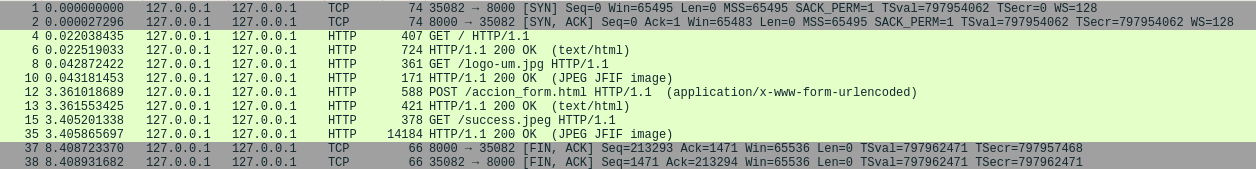
\includegraphics[width=0.95\textwidth]{tests/capture_normal.png}
    \caption{Intercambio de mensajes sin errores.}
    \label{img-cap-normal}
\end{figure}

\item [\cref{img-cap-malfunctioning}] Una prueba de algunos mensajes de error. Muestra un \key{404 Not Found} y un \key{415 Unsupported Media Type}. Además, también muestra la robustez del servidor. Ante un {\POST} de más de \SI{8}{\kibi\byte}, que hemos simulado introduciendo $9000$ caracteres en el campo del correo, devuelve un mensaje \key{413 Request Entity Too Large} y corta la conexión% a footnote
\footnote{Aunque como hemos explicado antes el servidor está preparado para procesar mensajes de tamaño arbitrario leyéndolos en bloques de \SI{8}{\kibi\byte}, hemos establecido el máximo en \SI{8}{\kibi\byte}.}
.

\begin{figure}[h]
    \centering
    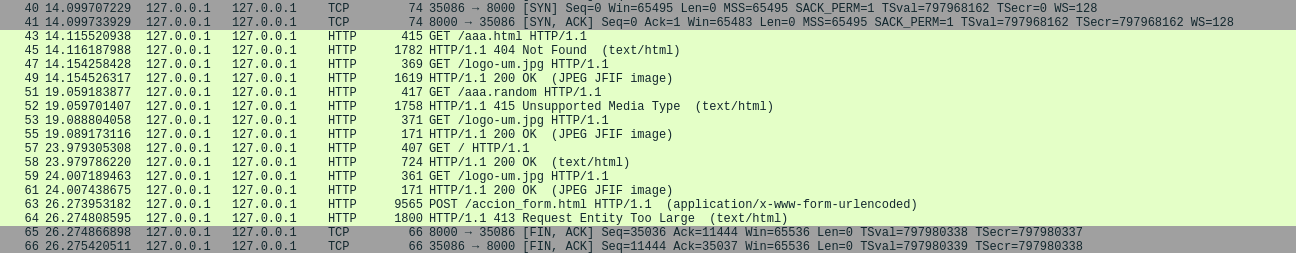
\includegraphics[width=0.95\textwidth]{tests/capture-malfunctioning.png}
    \caption{Intercambio de mensajes de error.}
    \label{img-cap-malfunctioning}
\end{figure}

\item [\cref{img-cap-pipelining}] Una captura probando que el servidor acepta \key{pipelining}. Como el navegador no hacía \key{pipelining}, lo hemos probado utilizando el script del \cref{lst-pipelining-shell}. En un solo paquete {\TCP} se reciben $4$ mensajes {\GET} que el servidor responde en orden. Mediante los mensajes de log se vio que los $4$ mensajes se leyeron en la misma operación de lectura.

\lstinputlisting[language=sh, float, label=lst-pipelining-shell]{tests/pipelining.sh}

\begin{figure}[h]
    \centering
    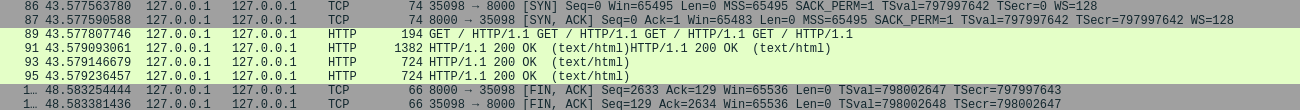
\includegraphics[width=0.95\textwidth]{tests/capture-pipelining.png}
    \caption{Prueba de \key{pipelining}.}
    \label{img-cap-pipelining}
\end{figure}

\end{itemize}


\section{Horas de Trabajo}
Para contabilizar las horas trabajadas en esta entrega hemos utilizado la herramienta \key{progesa-test} de la Facultad de Informática. A continuación se puede ver una tabla con el tiempo dedicado a cada apartado de la práctica.

\begin{center}
\begin{tabular}{|p{5cm}|c|}
    \hline
    \multicolumn{2}{|c|}{Entrega Anticipada} \\
    \hline\hline
    \multicolumn{1}{|c|}{Actividad} & Trabajo Autónomo \\
    \hline
    Implementación básica servidor {\HTTP} & \SI{17}{\hour} \SI{24}{\minute} \\
    \hline
    Documentación & \phantom{9}\SI{7}{\hour} \SI{39}{\minute} \\
    \hline
    Revisión & \phantom{\SI{99}{\hour}} \SI{35}{\minute} \\
    \hline
    \textbf{TOTAL} & \SI{25}{\hour} \SI{38}{\minute} \\ \hline
    % \textbf{MEDIAS} & 2.26\% & 5.45\% & 88.85\% & 3.43\% & 100\% \\ \hline
\end{tabular}
\end{center}


% \section{Conclusiones}
    % \lstinputlisting[caption=message\_processing.cpp]{../src/message_processing.cpp}
\end{document}
